\section{Einleitung}

Ziel der Arbeit im Rahmen der Vorlesung Robotik war es, das Spiel \glqq Vier Gewinnt\grqq ~auf einer LED-Matrix zu implementieren und eine Künstliche Intelligenz zu entwickeln, die es ermöglicht auch alleine das Spiel zu nutzen.

\section{Vier Gewinnt}
\label{sec:vierg}
Bei \glqq Vier Gewinnt\grqq ~handelt es sich um ein Spiel, bei dem zwei Spieler auf einem klassischerweise 6x7 Feld (6 Zeilen, 7 Spalten) versuchen über das jeweilige Setzen von Steinen eine Reihe von vier Steinen zu erzeugen. Die Vorraussetzungen dabei sind, dass der jeweilige Stein am unteren Ende der Spalte gesetzt wird und die Spieler stets nacheinander am Zuge sind.

\begin{figure}[!hbt]
	\centering
	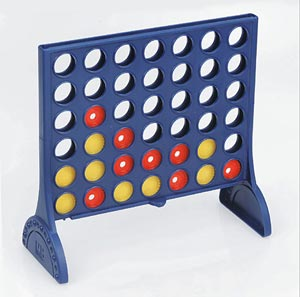
\includegraphics[scale=0.8]{4Gewinnt.jpeg}
	\caption{Ein klassisches Vier-Gewinnt-Spiel}
\end{figure}

Aus mathematischer Sicht ist \glqq Vier Gewinnt\grqq ~ein Spiel mit perfekter Information. Dies bedeutet, dass zu jedem Zeitpunkt alle vorhergehenden Züge bekannt sind. Diese perfekte Information sorgt dafür, dass das Spiel volständig gelöst ist. Daraus kann abgeleitet werden, dass der Ausgang des Spiels für zwei perfekt spielende Gegner davon abhängig ist, in welche Spalte der erste Stein gesetzt worden ist: Wurde der erste Stein in die mittlerste Spalte gesetzt, so gewinnt bei perfektem Spiel stets der erste Spieler. Beim Setzen in eine der Nachbarspalten, endet das Spiel unentschieden, sollte der erste Stein in eine der übrigen Spalten gesetzt werden, so gewinnt der zweite Spieler. 

\section{LED-Matrix und Darstellung des Spielfeldes}
Um \glqq Vier Gewinnt\grqq ~auf einer LED-Matrix abbilden zu können müssen zwei wesentliche Eigenschaften von der Matrix erfüllt werden: Zunächst muss die Matrix eine Mindestgröße von 6x7 besitzen, zum anderen muss sie fähig sein mindestens zwei unterschiedliche Farben abzubilden.
Bei der Suche nach einer geeigneten Matrix hat sich herausgestellt, dass vor allem die zweite Eigenschaft ein Problem darstellt.
Es konnte dennoch eine geeignete Matrix gefunden werden:
Das \glqq Adafruit 16x32 RGB LED matrix panel\grqq.

\begin{figure}[!hbt]
	\centering
	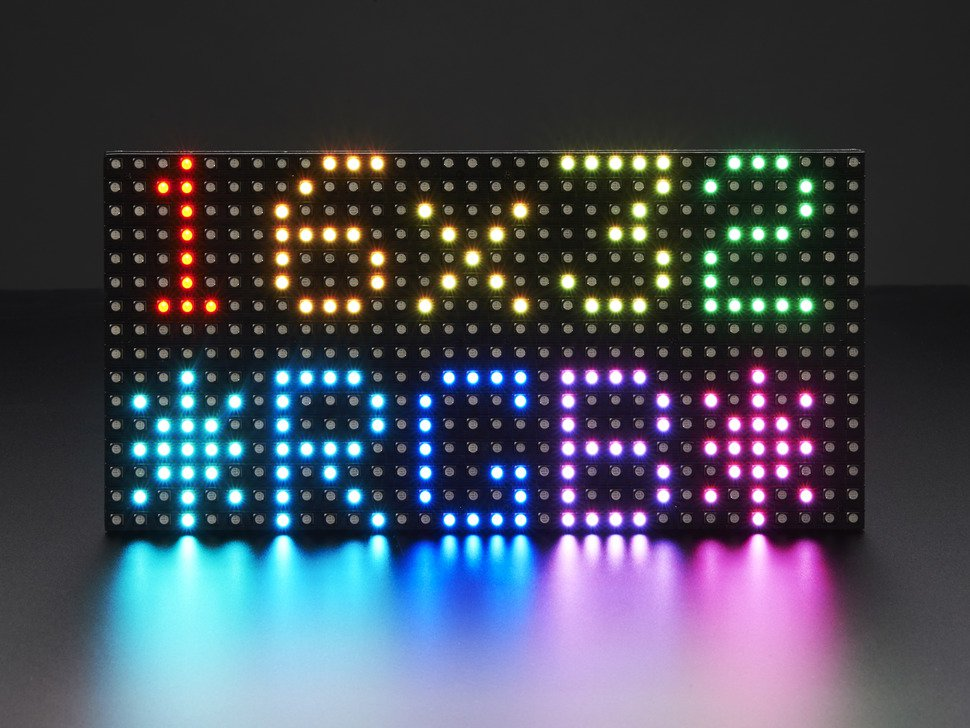
\includegraphics[scale=1]{RGBLEDMatrix.jpg}
	\caption{Verwendete LED-Matrix von Adafruit}
\end{figure}

Da die Matrix mit 16x32 deutlich über der Anforderung lag, wurde entschieden, dass auf der Matrix jeder Stein durch ein 2x2 Feld  dargestellt wird.
Das Feld würde somit eine Fläche von 12x14 einnehmen. Da somit immer noch genügend Platz vorhanden ist, und die Matrix mehr als zwei Farben anbietet, soll das Spielfeld durch einen Rand in einer anderen Farbe begrenzt werden.
Die somit ausgefüllte Fläche beträgt 14x16.
Zur besseren Visualisierung wurde zuletzt noch entschieden, über dem Spielfeld durch einen blinkenden Stein sowohl darzustellen, welcher Spieler aktuell am Zug ist, als auch in welche Spalte der nächste Stein aktuell gesetzt werden würde.
Insgesamt wird somit die Hälfte der Matrix genutzt, ein 16x16 Feld.
Aus ästhetischen Gründen wird daher das gesamte Feld in der Mitte der Matrix angezeigt.

\section{Künstliche Intelligenz}
Nachdem die Ansteuerung der Matrix mit Hilfe eines Python Skripts funktioniert, wurde noch eine Kümnstliche Intelligenz (KI) entwickelt, die anhand der gegebenen Informationen und Ressourcen in annehmbarer Zeit eine Zugentscheidung zu produzieren.
Wie in dem Kapitel \ref{sec:vierg} beschrieben handelt es sich bei \glqq Vier Gewinnt\grqq ~um ein Spiel mit perfekter Information handelt. Zusätzlich gehört das Spiel in die Kategorie der Nullsummenspiele. Dies bedeutet, dass die Gewinne und Verluste der beiden Spieler addiert stets 0 ergeben müssen.
Auf Grundlage dieser Informationen ist es möglich für eine KI den Minimax-Algorithmus einzusetzen.

Bei dem Minimax-Algorithmus handelt es sich um einen Gewinnoptimierungsalgorithmus, der über Heuristiken verschiedene Spielsituationen auswertet und den jeweilig besten Zug auswählt.
Für \glqq Vier Gewinnt\grqq ~muss der Algorithmus abgewandelt werden, da der Minimax-Algorithmus in seinen Grundzügen darauf optimiert ist einen maximierenden und einen minimierenden Spieler zu analysieren. Da bei \glqq Vier Gewinnt\grqq ~allerdings beide Spieler maximieren, muss bei der Analyse jeweils darauf geachtet werden, dass das Ergebnis des letzten Spielers negiert wird. Diese Abwandlung wird auch Negamax-Algorithmus genannt.

\begin{algorithm}
\caption{Negamax-Algorithmus}
\begin{algorithmic}[1]
\Procedure{NegaMax}{player, depth}
\If {$ depth == 0$~\textbf{or}~$\textit{noPlayableTurns}$} 
\State \Return $\textit{score(player)}$
\EndIf
\State $\textit{maxValue} \gets -\textit{infinity}$
\State $\textit{getPlayableTurns()}$
\While {$\textit{movableTurnsLeft}$}
\State $\textit{makeTurn()}$
\State $\textit{value} \gets -\textit{NegaMax(otherPlayer, depth-1)}$
\State $\textit{redoTurn()}$
\If {$\textit{value} \textgreater \textit{maxValue}$}
\State $\textit{maxValue} \gets \textit{value}$
\If {$\textit{depth} = \textit{requiredDepth}$}
\State $\textit{savedTurn} \gets \textit{turn}$
\EndIf
\EndIf
\EndWhile
\State \Return $\textit{maxValue}$
\EndProcedure
\end{algorithmic}
\end{algorithm}